\documentclass[xcolor=dvipsnames]{beamer}
%\documentclass[handout,xcolor=dvipsnames]{beamer}
%\documentclass[handout,xcolor=dvipsnames,pdftex,hyperref={colorlinks=false}]{beamer}

% == Packages for beamer
\usepackage{xcolor}
\usepackage{graphicx}
\graphicspath{{images/}{figures/}}
\usepackage{fancybox}
\usepackage{hyperref}
\usepackage{amsmath,amssymb,amsfonts,bm}
\usepackage{wasysym}

\usepackage[english]{babel}
\usepackage{times}
\usepackage[T1]{fontenc}

% == Other Packages
\usepackage{rotating}
\usepackage{latexsym}
\usepackage{ulem}


% == theme & colors
\usetheme{Warsaw}  % Jens' previous
\usepackage{helvet}
\definecolor{someblue}{rgb}{0,.1,0.8}

% == New Commands
% = For general typesetting
\newcommand\spacingset[1]{\renewcommand{\baselinestretch}{#1}\small\normalsize}
\renewcommand\r{\right}
\renewcommand\l{\left}

\newcommand\makegaps{\addtolength{\itemsep}{.25\baselineskip}}
\newcommand\makebiggaps{\addtolength{\itemsep}{.5\baselineskip}}

% = For stats & econometrics
\renewcommand{\epsilon}{\varepsilon}
\newcommand\ud{\mathrm{d}}
\newcommand\dist{\buildrel\rm d\over\sim}
\newcommand\ind{\stackrel{\rm indep.}{\sim}}
\newcommand\iid{\stackrel{\rm i.i.d.}{\sim}}
\newcommand\logit{{\rm logit}}
\newcommand\cA{\mathcal{A}}
\newcommand\cN{\mathcal{N}}
\newcommand\E{\mathbb{E}}
\newcommand\V{\mathbb{V}}
\newcommand\cJ{\mathcal{J}}
\newcommand\y{{\bm y}}
\newcommand\Y{{\bm Y}}
\newcommand\X{{\bm X}}
\newcommand\x{{\bm x}}
\newcommand\eps{{\bm\varepsilon}}
\newcommand\zero{{\bm 0}}
\newcommand\be{{\bm\beta}}
\renewcommand\b{{\bm b}}
\newcommand\C{{\bm C}}
\newcommand\D{{\bm D}}
\newcommand\I{{\bm I}}
\newcommand\Z{{\bm Z}}
\newcommand\eeta{{\bm \eta}}
\DeclareMathOperator*\plim{plim}
\DeclareMathOperator\rank{rank}
\newcommand\indep{\protect\mathpalette{\protect\independenT}{\perp}}
\DeclareMathOperator{\sgn}{sgn}
\def\independenT#1#2{\mathrel{\rlap{$#1#2$}\mkern2mu{#1#2}}}

%\documentclass[xcolor=dvipsnames]{beamer}
%%\usecolortheme[named=OliveGreen]{structure}
%\usecolortheme[named=Blue]{structure}
%%\usetheme{Rochester}
%\setbeamertemplate{items}[ball]
%\setbeamertemplate{blocks}[rounded][shadow=true]
%\usepackage{xcolor}
%\usepackage{colortbl}
%\setbeamertemplate{navigation symbols}{}
%\usepackage{amssymb}
%\usepackage{amsmath}
%\usepackage[english]{babel}
%% or whatever
%
%%\usepackage[latin1]{inputenc}
%% or whatever
%
%%\mode<presentation>
%%{
%\usetheme{Warsaw}
%  % or ...
%  %\usecolorheme{albatross}
%%  \setbeamercovered{transparent}
%  % or whatever (possibly just delete it)
%%}

%\usepackage{helvet}
%%\usepackage[T1]{fontenc}
%% Or whatever. Note that the encoding and the font should match. If T1
%% does not look nice, try deleting the line with the fontenc.

%\newcommand{\indep}{{\bot\negthickspace\negthickspace\bot}}
\newcommand{\notindep}{{\bot\negthickspace\negthickspace\bot}{\negthinspace
  \negmedspace \negthickspace \negthickspace \diagup
  \;}}

\newcommand{\bs}{\boldsymbol}
\newcommand{\mb}{\mathbf}
\newcommand{\real}{\mathbb{R}}
\renewcommand{\u}{\ensuremath{\mb{u}}}
\renewcommand{\v}{\ensuremath{\mb{v}}}
\newcommand{\U}{\ensuremath{\mb{U}}}
\newcommand{\M}{\ensuremath{\mb{M}}}
\renewcommand{\b}{\ensuremath{\bs{\beta}}}
\newcommand{\e}{\ensuremath{\bs{\epsilon}}}
\newcommand{\bhat}{\ensuremath{\hat{\bs{\beta}}}}
\newcommand{\XX}{\ensuremath{\X'\X}}
\newcommand{\XXinv}{\ensuremath{\left(\XX\right)^{-1}}}
\newcommand{\hatsig}{\ensuremath{\hat{\sigma}^2}}
\newcommand{\sig}{\ensuremath{\sigma^2}}
\newcommand{\hatmat}{\ensuremath{\X \XXinv \X'}}
\newcommand{\ehat}{\ensuremath{\hat{\e}}}
\newcommand{\tr}{\text{tr}}
\newcommand{\Sig}{\ensuremath{\bs{\Sigma}}}
\newcommand{\SigInv}{\ensuremath{\bs{\Sigma^{-1}}}}
\newcommand{\W}{\ensuremath{\mb{W}}}

\title[]{The Potential Outcome Framework}
\subtitle[ ]{PS200C, Causal Inference, Spring 2026}
\author[Hazlett]{Chad Hazlett }
\institute[UCLA]{UCLA\\[1ex]
  \texttt{chazlett@ucla.edu}
}
\date{}

\definecolor{dgreen}{rgb}{0,.6,0.8}
\newtheorem{assumption}{Assumption}
\useoutertheme{infolines}
\begin{document}

\subject{Talks}
\AtBeginSection[]
{
  \begin{frame}<beamer>
    \frametitle{Outline}
    \tableofcontents[currentsection]
  \end{frame}
}

\AtBeginSubsection[]
{
  \begin{frame}<beamer>
    \frametitle{Outline}
    \tableofcontents[currentsection,currentsubsection]
  \end{frame}
}

\begin{frame}
  \titlepage
%\begin{block}{While we wait,...}
%  \begin{itemize}
%  \item Are we recording?  \end{itemize}
%\end{block}
\end{frame}

\begin{frame}{What is causality?}
\begin{center}
What do we mean when we say $X$ causes $Y$, or $Y$ was caused by $X$? \\

\bigskip
\bigskip

Thoughts?
\end{center}
\end{frame}


\begin{frame}
Reading: Chapers 1 and 2 from ``What If" (Hernan \& Robins)
\end{frame}

\begin{frame}{Flavors of causality}
  
\onslide<1-> \textbf{Effect of causes.} One kind of causal question the most common type of causal question in applied areas-regards the \textit{effect} of some potential cause, e.g. what is the effect of:\\
\medskip
\footnotesize
\begin{itemize}
 \item political institutions on corruption?
 \item effect of a drug or other therapy on a health outcome
 \item an ad on purchasing behavior
 \item peace-keeping missions on peace?
 \item body cameras on police behavior?
\end{itemize}
\normalsize
\onslide<2-> \textbf{Causes of effects/ causal attribution}. Another set of questions asks ``what led to an observed outcome''.\\
\bigskip
\onslide<3-> Other/more general/complicated concepts can be embedded in a deep enough framework (namely structural causal models)
\end{frame}

\begin{frame}{Two languages}
Most work on causality now employs one of two languages:

\begin{figure}
\begin{minipage}{.5\textwidth}
  \centering
  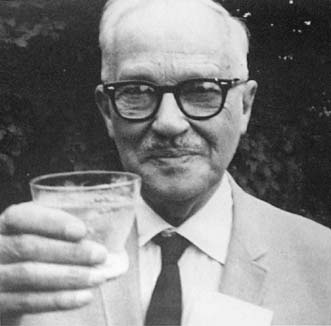
\includegraphics[width=.4\linewidth]{images/Neyman_3.jpeg}
    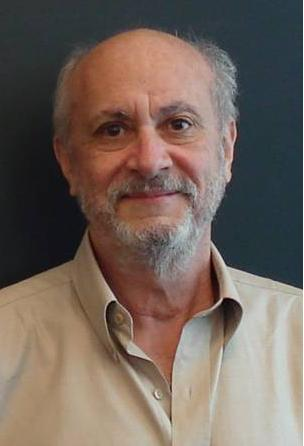
\includegraphics[width=.27\linewidth]{images/DonRubin.jpg}
  \caption{Neyman and Rubin}
\end{minipage}%
\begin{minipage}{.5\textwidth}
  \centering
    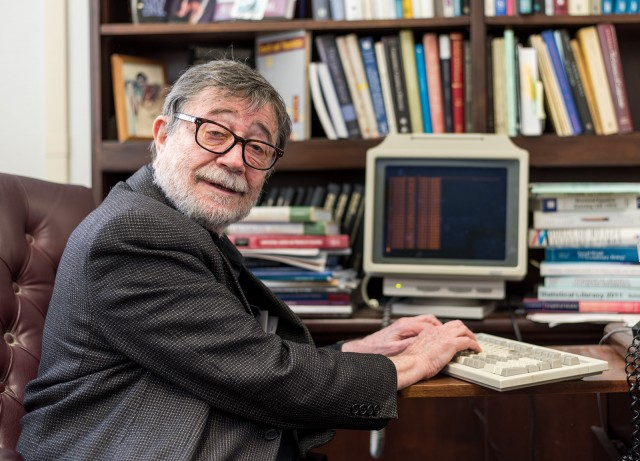
\includegraphics[width=.6\linewidth]{images/pearl.jpg}
  \caption{Judea Pearl}
\end{minipage}
\end{figure}
\small
\begin{itemize}
\item  \textcolor{Blue}{Neyman-Rubin causal model}, aka the \textcolor{Blue}{Potential Outcomes Model} (POM). 
\item Pearl associated with structural causal models (SCMs), graphs (directed acyclic graphs, DAGs)
\end{itemize}

\onslide<2-> We will use both extensively, but start with potential outcomes.
\end{frame}

\begin{frame}{A Running Example}
\onslide<1-> \textbf{Research question}: Does getting a college degree make people more politically liberal? \\
\bigskip
\begin{itemize}
\item<2-> \textbf{Treatment} ($D_i$): Completing a college degree (vs.\ not)
\item<3-> \textbf{Outcome} ($Y_i$): Liberal attitudes (e.g.\ a policy liberalism scale)
\item<4-> \textbf{Confounders to imagine}:
\begin{itemize}
\item Parental income and education
\item Urban vs.\ rural upbringing
\item Pre-existing political attitudes
\end{itemize}
\end{itemize}
\bigskip
\onslide<5-> We'll use this example throughout to make the abstract machinery concrete.
\end{frame}

\begin{frame}{What Causal Inference Actually Asks}
\onslide<1-> \textbf{What we do naturally:}
\begin{itemize}
\item Split people into a treated group and a control group
\item Compare average outcomes across groups
\item ``College grads are more liberal than non-grads''
\end{itemize}
\bigskip
\onslide<2-> \textbf{What causal inference asks:}
\begin{itemize}
\item For each person, compare how they would do \textit{if treated} to how they would do \textit{if untreated}
\item ``Would \textit{this person} be more liberal \textit{if they got a degree} than \textit{if they didn't}?''
\end{itemize}
\bigskip
\onslide<3-> The first is a comparison between groups of different people. The second is a comparison within each person, between two versions of their life.
\end{frame}

\begin{frame}{What Causal Inference Actually Asks}
\begin{center}
  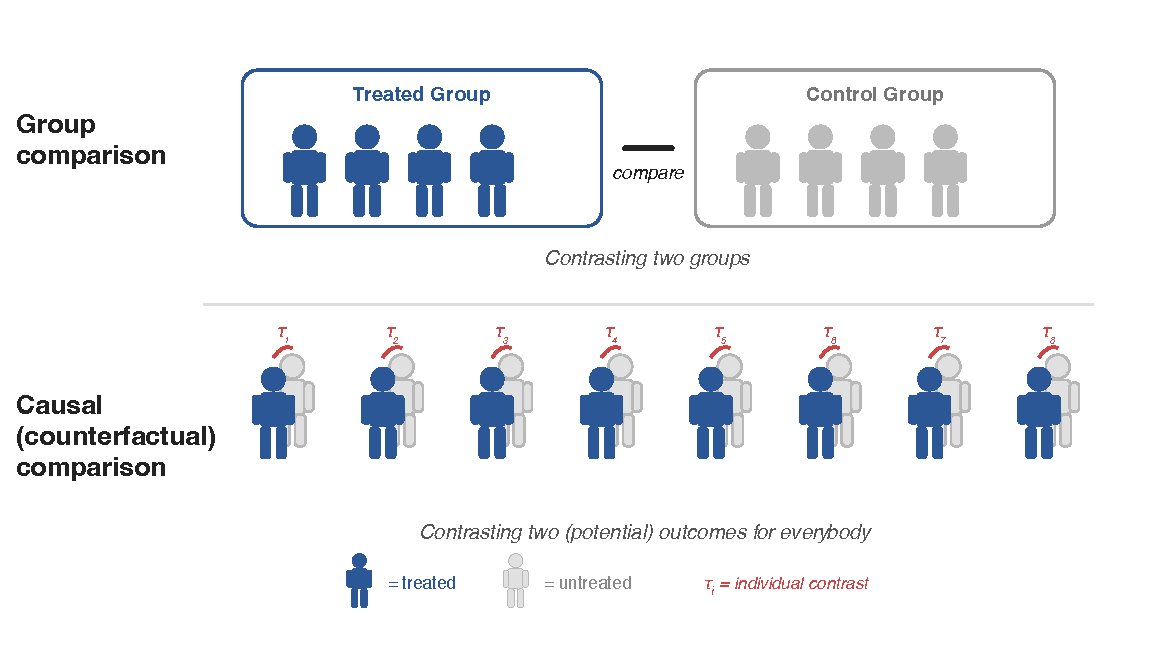
\includegraphics[width=\textwidth]{images/group_vs_counterfactual.pdf}
\end{center}
\end{frame}

\begin{frame}{Potential Outcomes Notation}
\vspace{-.05in}
\begin{center}
  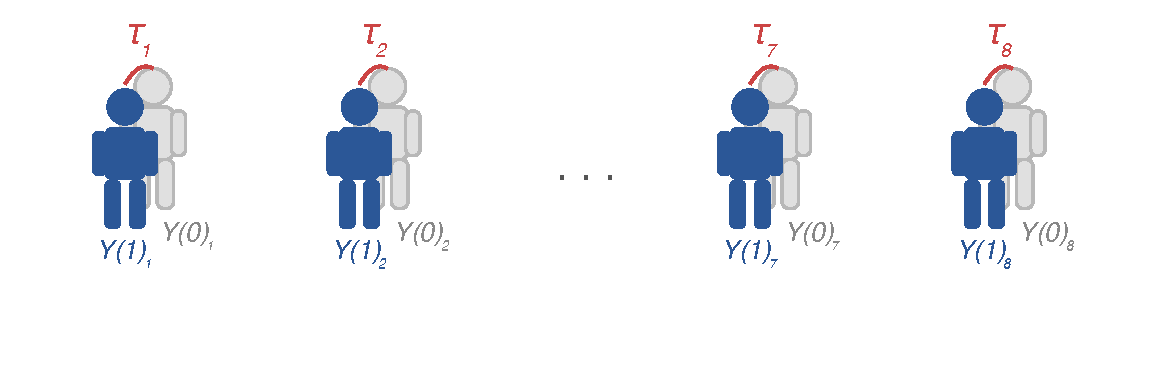
\includegraphics[width=\textwidth]{images/counterfactual_labeled.pdf}
\end{center}
\vspace{-.25in}
\small
\begin{itemize}
\item $\textcolor{Blue}{Y_i(1)}$: the outcome unit $i$ \textit{would have} under treatment
\item $\textcolor{Gray}{Y_i(0)}$: the outcome unit $i$ \textit{would have} under control
\item $\textcolor{Red}{\tau_i} = Y_{1i} - Y_{0i}$: the causal effect for unit $i$
\item Sample average causal effect: $\;\frac{1}{n}\sum_{i=1}^{n} \tau_i = \frac{1}{n}\sum_{i=1}^{n} \left(Y_{1i} - Y_{0i}\right)$
\end{itemize}
\medskip
The  \textcolor{Red}{fundamental problem of causal inference}: you only get to see \textit{one} potential outcome per unit. We need assumptions to somehow "fill in the missing'' potential outcome.
\end{frame}

\begin{frame}{From Potential Outcomes to Observed Data}
\small
Now add the treatment indicator $D_i$ (1 if treated, 0 if not). Key insight: \textit{treatment doesn't change the potential outcomes---it changes which one you see}:
\[Y_i = D_i \, Y_i(1) + (1-D_i) \, Y_i(0)\]
\medskip
\onslide<2-> Which of these are \textcolor{blue}{always observable}, \textcolor{blue}{sometimes observable}, or \textcolor{blue}{never observable}?\\

\begin{enumerate}
\item<3-> $Y_i(1)$ and $Y_i(0)$ (at the same time, for the same unit)
\item<4-> $D_i$
\item<5-> $Y_i$
\item<6-> $\tau_i$
\end{enumerate}
\end{frame}

\begin{frame}{Quantities of Interest}
\footnotesize
\begin{itemize}
\item<1-> Average Treatment Effect (ATE):
\[ATE = \E[Y_{i}(1)-Y_{i}(0)] = \E[\tau_i] \]
\item<2-> Average treatment effect on the treated (ATT):
\[ATT = \E[Y_{i}(1)-Y_{i}(0)|D_i=1]\]
\item<3-> Average treatment effect on the controls (ATC):
\[ATC = \E[Y_{i}(1)-Y_{i}(0)|D_i=0]\]
\item<4-> Average treatment effect for sub-groups ($ATE(X)$):
\[ATE(X) = \E[Y_{i}(1)-Y_{i}(0)|X_i=x]\]
\end{itemize}
\end{frame}

\begin{frame}{Visualizing the ATT}
\small
The ATT asks: among units who were actually treated ($D_i=1$), what is the average of their individual causal effects? \\
\smallskip
Not a group comparison---imagine each treated unit's two potential lives:
\begin{center}
  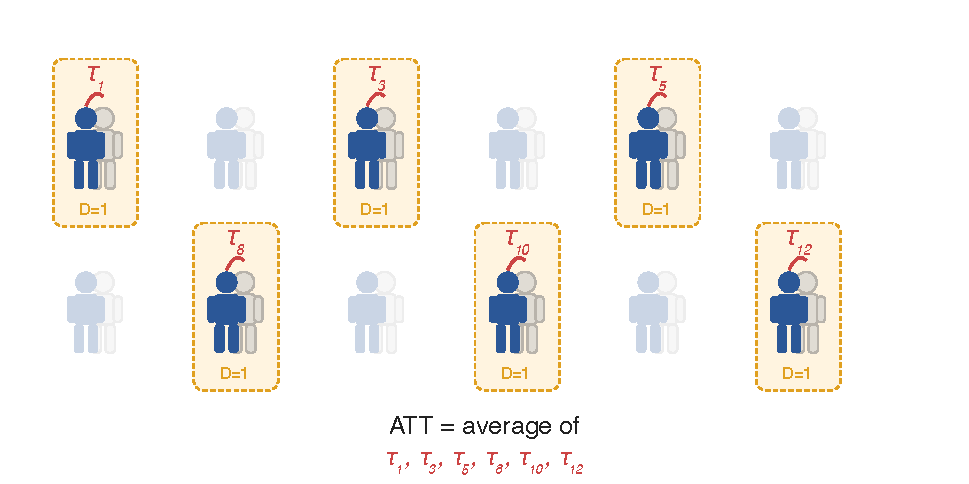
\includegraphics[width=0.85\textwidth]{images/att_visual.pdf}
\end{center}
\end{frame}

\begin{frame}{Visualizing the ATC}
\small
The ATC asks the same question for the untreated ($D_i=0$): \\
\smallskip
These units were \textit{not} treated, but we still ask what \textit{would have happened} if they had been:
\begin{center}
  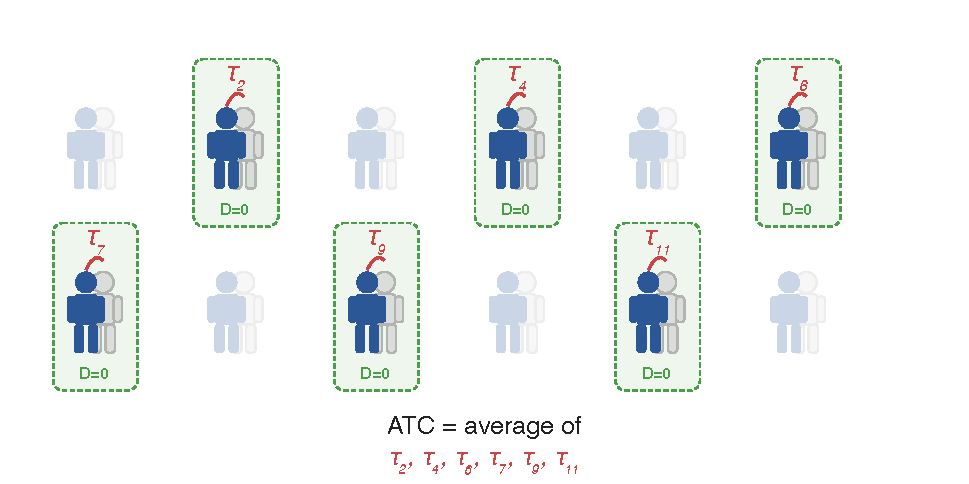
\includegraphics[width=0.85\textwidth]{images/atc_visual.pdf}
\end{center}
\end{frame}

\begin{frame}{The one embodied assumption: Consistency}
\small
\onslide<1-> By writing $Y_i(d)$ we assert \textbf{consistency}: $Y_i(d)$ is the $Y_i$ you'd see if $i$ received treatment $d$.\\
\medskip
\onslide<2-> Worrying about consistency:
\footnotesize
\begin{itemize}
\item<3-> \textbf{Interference}: other units' treatment affects $i$'s outcome, so $Y_i(d)$ is not well-defined without specifying everyone else's status. Problematic. 
\medskip
\item<4-> \textbf{Treatment variation}: treatment may differ across units (e.g.\ which project a village picks in a CDD program). This is not usually a problem---variation only threatens consistency if it differs systematically by assignment, which is handled by randomization or identification assumptions later.
\end{itemize}
\small
\onslide<5-> You will encounter \textbf{SUTVA} (Rubin 1980) = no interference + ``one version of treatment.''\\
\begin{itemize}
\item These are threats to consistency, \textit{not additional assumptions}, don't go listing assumptions for no reason.
\end{itemize}
\end{frame}

\begin{frame}{Problematic POs}
\onslide<1-> Just because you can write a PO doesn't mean you should.\\
\footnotesize
\begin{itemize}
\item<2-> With a PO we imagine changing the treatment status of a unit. If you cannot imagine how you would intervene, it may signal ill-definedness.
\end{itemize}
\small
\onslide<3-> Example: what is the effect of leader gender on some outcome? \\
\footnotesize
\begin{itemize}
\item<3-> For US presidents, this involves $Y_{trump}(female)$, i.e. ``What would Donald Trump have done if he was female?''
\item<4-> ``Changing Trump to female'' would change countless subsequent experiences (and the probability of being in the sample of presidents anyway).
\end{itemize}
\small
\onslide<5-> Similarly, a concept may seem modifiable yet we may be unclear about what exactly it would change (e.g.\ the effect of obesity on health).
\end{frame}



\begin{frame}{Train your brain}
\onslide<1-> \textbf{Test 1}: Is $\E[Y_{1i}|D_i=1]=\E[Y_i|D_i=1]$?\\
\medskip
\onslide<2-> What licenses it?
\end{frame}

\begin{frame}{Train your brain}
\onslide<1-> \textbf{Test 2}: Someone is assigning $D_i$ at random. 
\small
\begin{itemize}
\item<2-> What can we say about $\E[Y_{1i}|D_i=1]$ compared to $\E[Y_{1i}|D_i=0]$ and $\E[Y_{1i}]$?
\bigskip
\item<3-> What would $\E[Y_i|D_i=1]-\E[Y_i|D_i=0]$ tell us?
\end{itemize}
\end{frame}


\begin{frame}{Train your brain}
%\onslide<1-> \textcolor{Blue}{Recall $D_i$ is a ``switch'' that determines whether you see $Y_{1i}$ or $Y_{0i}$} \\
%\bigskip 
\onslide<1-> \textbf{Test 3}: Suppose $Y_{1i}=Y_{0i}$ for all $i$ (no effect). But someone assigns $D_i=1$ more often when $Y_{1i}$ is higher.
\small
\begin{itemize}
\item<2-> Does $\E[Y_{1i}|D_i=1]=\E[Y_{1i}|D_i=0]$?
\medskip
\item<3-> If you estimated $\E[Y_i|D_i=1]-\E[Y_i|D_i=0]$, do you expect zero, positive, or negative?
\medskip
\item<4-> What is the direction of bias, and why?
\end{itemize}
\end{frame}

\begin{frame}{Train your brain}
\onslide<1-> \textbf{Test 4}: Suppose you don't know anything about how $D_i$ is assigned w.r.t. $Y_{1i}$ and $Y_{0i}$. 
\begin{itemize}
\item<2-> Can we say anything about how $\E[Y_1i|D=1]$ compares to $\E[Y_1i]$?
\bigskip
\item<3-> Can we say anything about how $\E[Y_0i|D=0]$ compares to $\E[Y_0i]$?
\bigskip
\item<4-> So can we say anything about how $\E[Y_i|D_i=1]-\E[Y_i|D_i=0]$ compares to $\E[Y_{1i}-Y_{0i}]$?
\end{itemize}
\bigskip
\normalsize
\begin{center}
\alert{\onslide<5-> Which of these scenarios are we usually in with observational data?}
\end{center}
\end{frame}

\begin{frame}{Visual Practice}
\small
\onslide<1-> Let's looks at $Y_{1i}$ and $Y_{0i}$ alone first. \\
\vspace{-.4in}
\begin{center}
  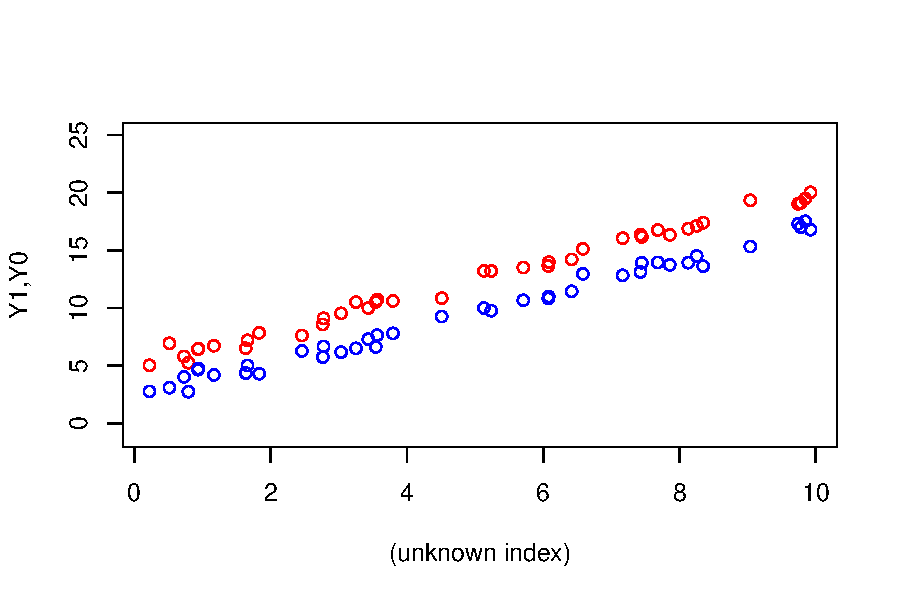
\includegraphics[scale=.7]{y0y1plot_blank.pdf} 
\end{center}
\vspace{-.2in} 
\onslide<1-> True $\E[Y_{1i}-Y_{0i}]=ATE=3$\\
%\medskip
%\onslide<1-> %$\overline{Y}_{1i}-\overline{Y}_{0i}=\hat{ATE}=3.01$\\
\end{frame}

\begin{frame}{Random Assignment of Treatment}
\small
\onslide<1-> Now suppose $D_i=1$ is randomly assigned. We see only the filled dots:\\
\vspace{-.4in}
\begin{center}
  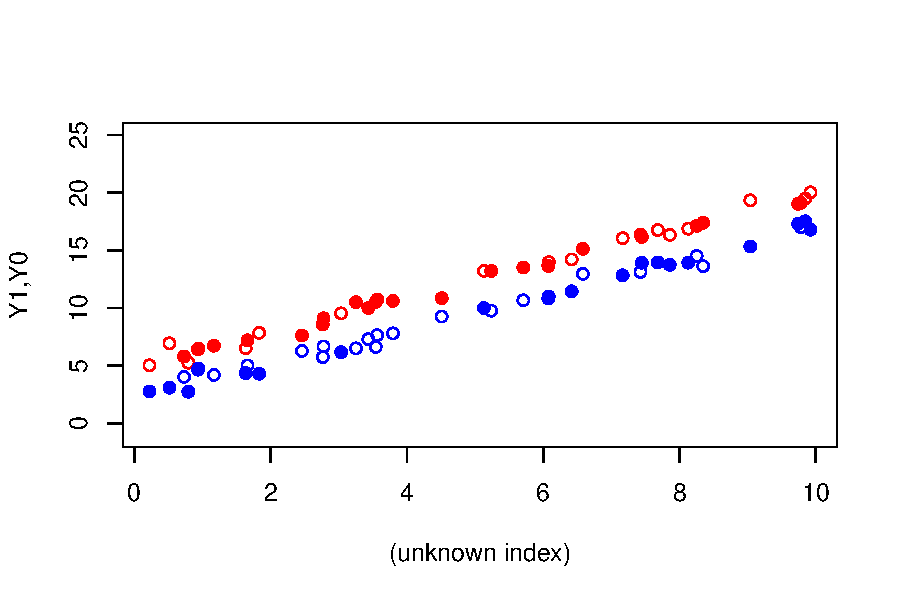
\includegraphics[scale=0.7]{y0y1plot_nobias.pdf}\\
\end{center}
\vspace{-.2in}
\onslide<2-> We get \[\hat{\E}[Y_i|D_i=1]-\hat{\E}[Y_i|D_i=0]=\widehat{ATE}=3.01\]
\end{frame}

\begin{frame}{Non-Random Assignment of Treatment 1}
\small
\onslide<1-> Suppose $Pr(D_i=1)$ increases to the right. Now we observe (filled dots):\\
\vspace{-.4in}
\begin{center}
  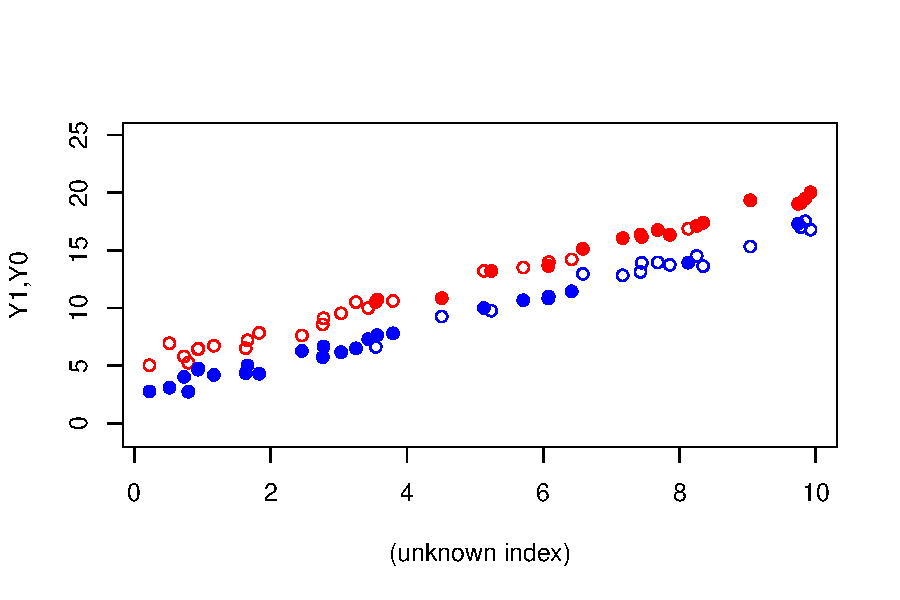
\includegraphics[scale=0.7]{y0y1plot_posbias.pdf}\\
\end{center}
\vspace{-.2in}
\onslide<2-> What difference in means do you expect?\\
\vspace{-.1in}
\onslide<3-> \[\hat{\E}[Y_i|D_i=1]-\hat{\E}[Y_i|D_i=0]=\widehat{ATE}=9.97\]
\end{frame}

\begin{frame}{Non-Random Assignment of Treatment 2}
\small
\onslide<1-> Now suppose $Pr(D_i=1)$ decreases to the right. We observe (filled dots):\\
\vspace{-.5in}
\begin{center}
  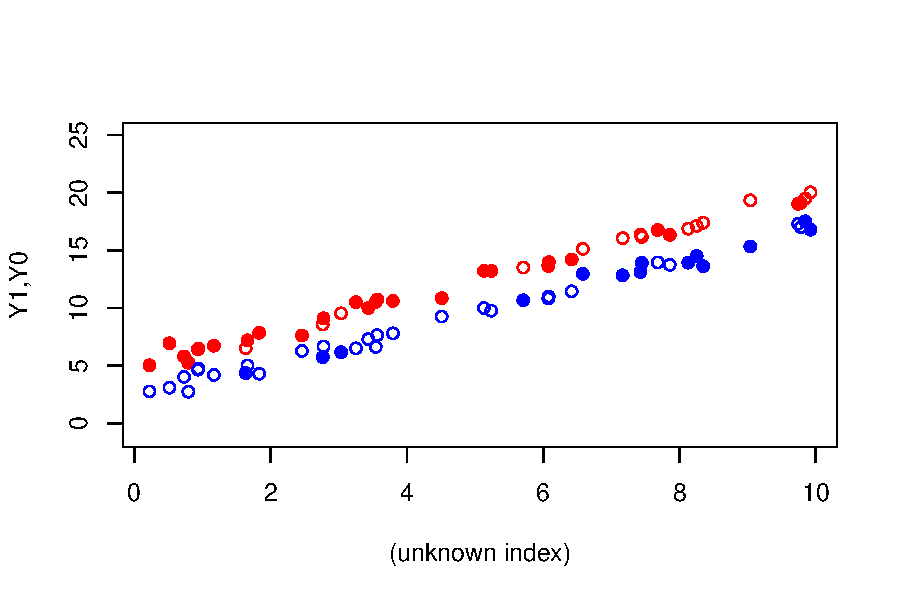
\includegraphics[scale=0.7]{y0y1plot_negbias.pdf}\\
\end{center}
\vspace{-.3in}
\onslide<2-> What difference in means do you expect now?
\vspace{-.05in} \onslide<3-> \[\hat{\E}[Y_i|D_i=1]-\hat{\E}[Y_i|D_i=0]=\widehat{ATE}=-1.59\] \\
\onslide<4-> What can we do about this? \onslide<5-> \textcolor{Blue}{Nothing, yet}
\end{frame}

\begin{frame}{Preview: what if we observe a confounder?}
\footnotesize
\onslide<1-> Again $Pr(D_i=1)$ decreases to the right, but now suppose $X$ is observable and $D$ is random conditional on $X$. Compare treated to control at the same $X$:\\
\vspace{-.4in}
\begin{center}
  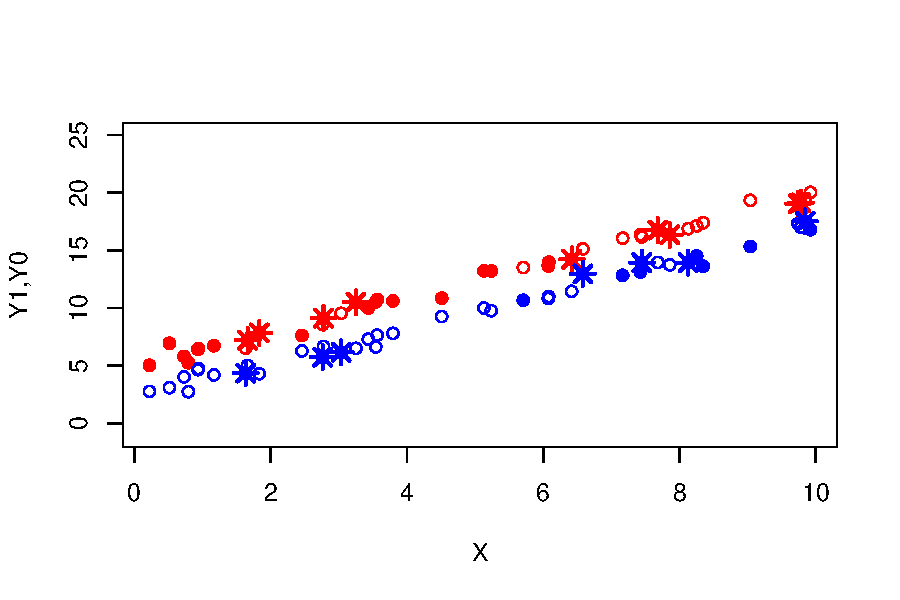
\includegraphics[scale=0.6]{y0y1plot_matched.pdf}\\
\end{center}
\vspace{-.2in}
\onslide<2->
\[[\overline{Y}_i|D=1]-[\overline{Y}_{i}|D=0]=\widehat{ATE}=2.63\]
\end{frame}


\begin{frame}{More PO practice: the ``science table''}
Imagine a study population with 4 units:

\begin{table}[ht]
    \centering
    \begin{tabular}{c  c c c c }
      $i$ & $D_i$ & $Y_{1i}$ & $Y_{0i}$ & $\tau_i$ \\ \hline
      1  & 1 & 10  & 4 & 6 \\
      2  & 1 & 1  & 2 & -1 \\
      3 & 0 & 3 & 3 & 0 \\
      4 & 0 & 5 & 2 & 3 \\
    \end{tabular}
    \end{table}

\onslide<2-> 1. What is the ATE?
\onslide<3-> \small $\E[Y_{1i} - Y_{0i}] = 1/4 \times (6-1+0+3)=2$ \\
\medskip
\footnotesize(Note: average effect is positive, but not all $\tau_i$ are)\\
\small
\medskip
\onslide<4-> 2. What are the ATT and ATC? \\
\begin{itemize}
\item<5->[] $\E[Y_{1i}-Y_{0i}|D_i=1]=.5(6-1)=2.5$\\
\item<6->[] $\E[Y_{1i}-Y_{0i}|D_i=0] =.5(0+3)=1.5$
\end{itemize}
\end{frame}

\begin{frame}{Naive Comparison: Difference in Means}
\small
\onslide<1-> You saw earlier how simple comparison of observed outcomes can be misleading. Let's use POM to see this more rigorously. \\
\bigskip
\onslide<2-> The \textcolor{Blue}{Difference in Means} estimand is $$\E[Y_i|D_i=1]-\E[Y_i|D_i=0]$$ \\
\bigskip
\onslide<3-> POM helps us compare this to QOIs. One terrific decomposition:

\footnotesize
\begin{align*}
\E[Y_i|D_i=1]-\E[Y_i|D_i=0] &= \E[Y_{1i}|D_i=1]-\E[Y_{0i}|D_i=0] \\
%&= \textcolor{Blue}{\E[Y_{1i}|D_i=1]-\E[Y_{0i}|D_i=1]} + \textcolor{Green}{\left(\E[Y_{i0}|D_i=1]-\E[Y_{0i}|D_i=0] \right)} \\
&= \textcolor{Blue}{\E[Y_{1i}-Y_{0i}|D_i=1]} + \textcolor{Green}{\left(\E[Y_{0i}|D_i=1]-\E[Y_{0i}|D_i=0] \right)}
\end{align*}
\small
\onslide<4-> What are the terms in \textcolor{Blue}{blue} \& \textcolor{Green}{green}?

%\begin{scriptsize}
%\begin{align}
%\begin{split}
%E[Y_i|D=1]-E[Y_i|D_i=0] \\
%&=E[Y_{1i} | D_i=1]-E[Y_{0i} | D_i=0]\\
%                 &=\underbrace{E[Y_{1i} - Y_{0i} | D_i=1]}_{\mbox{ATT}}
%                 +\underbrace{\{ E[Y_{i0} | D_i=1]- E[Y_{0i} | D_i=0]\}}_{\mbox{BIAS}}\nonumber
%\end{split}
%\end{align}
%\end{scriptsize}
%
%\begin{itemize}
%\itemsep1pt\parskip0pt\parsep0pt
%\item
%  Bias term unlikely to be 0 in most applications.
%\item
%  Selection into treatment is often associated with the potential
%  outcomes
%\end{itemize}
\end{frame}

\begin{frame}{Selection bias: examples}
\small
Recall: $\text{DIM} = \textcolor{Blue}{\text{ATT}} + \textcolor{Green}{\text{selection bias}}$, where \textcolor{Green}{$\text{bias}=\E[Y_{0i}|D_i=1]-\E[Y_{0i}|D_i=0]$}.\\
\bigskip
\onslide<2-> Example: $D=\text{Church Attendance}$, $Y=\text{Political Participation}$ \\
\footnotesize
\begin{itemize}
\item Church goers may already differ from non-goers (e.g.\ civic duty). So \textcolor{Green}{bias $\neq 0$}.
\end{itemize}
\smallskip
\small
\onslide<3-> Example: Human rights treaties\\
\footnotesize
\begin{itemize}
\item Countries willing to sign may already have better human rights. So \textcolor{Green}{bias $\neq 0$}.
\end{itemize}
\bigskip
\small
\onslide<4-> Our running example: $D=\text{College degree}$, $Y=\text{Liberal attitudes}$\\
\footnotesize
\begin{itemize}
\item People who get degrees may already be more liberal (parental education, urban upbringing). So \textcolor{Green}{bias $\neq 0$}.
\end{itemize}
\end{frame}

\begin{frame}{Assignment mechanism}
\small
\onslide<1-> We often start an analysis by thinking about how units are assigned to treatment. \\
\medskip
\onslide<2-> We can classify many important examples (similar to the graphical examples we tried) by what we know of the assignment mechanism (for $D_i$):
\footnotesize
\begin{itemize}
\item When we know it was random, we know those with $D=1$ and $D=0$ are ``comparable'', meaning same average POs. 
\smallskip
\item We previewed that if $D$ is random conditionally on observed $X$, we can manage.
\smallskip
\item When we don't know anything about assignment, \textcolor{Blue}{the data say nothing about the causal effects without importing some other assumption}.
\end{itemize}
\small
\medskip
\onslide<4-> Those represent important assignment mechanisms with hallowed names in varied fields: 
\footnotesize
\begin{itemize}
\item random assignment, ignorability, or exchangeability 
\item selection on observables, conditional ignorability
\item bad news
\end{itemize}
\end{frame}


\begin{frame}{What's next}
\begin{center}
\textcolor{Blue}{From here}: random assignment, then random-conditional-on-observables.
\end{center}
\end{frame}


\end{document} 